\chapter{RESULT}\label{cha:result}
TODO!

% ========== GYROTION TEST ==========
\section{Result Accelerometer \& Gyroscope-test}
As described in section ~\ref{sec:test:motion}, two test have been preformed on the accelerometer and gyroscope data with the result presented here.
\subsection{Test I}
The first test data were gathered from the web-page in \figureref{fig:gyrotion}, the result was around a hundred recordings from different devices. When looking at devices with similar or same hardware you can see differences in measurements, for example here are the accelerometer recordings from 5 iPhone 6 and 1 iPhone 5S:
\begin{figure}[H]
\centering
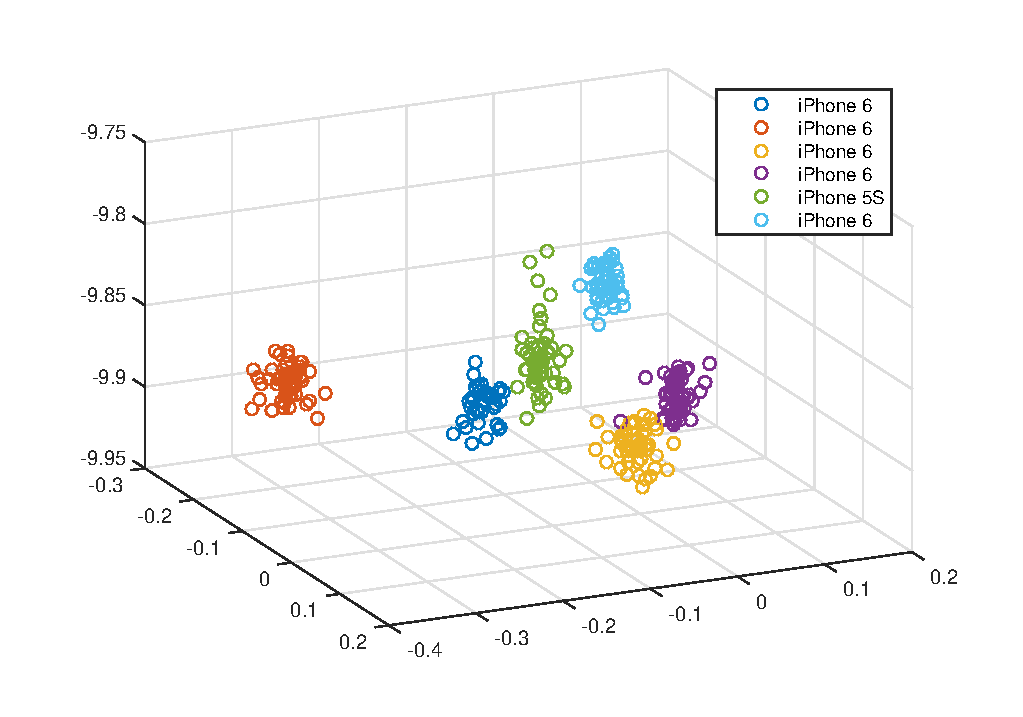
\includegraphics[scale=.7]{img/scatteriPhone}
\caption{Scatter graph on accelerometer recordings of 6 Apple devices}
\label{fig:digraph}
\end{figure}
The conclusions made from this scatters where that there may be were some calibration errors unique to each device. If that were the case the mean value from each recoding together with some kind of threshold could be enough for identifying each device based on accelerometer data. Just like the research made by \cite{sensor:micSpek}. 

\subsection{Test II}
TODO!

% ========== CAMERA TEST ==========
\section{Result Camera-test}
In section ~\ref{sec:test:camera} i descibed two test preformed on the camera sensor of mobile devices.
\subsection{Test I}
TODO!
\subsection{Test II}
TODO!

\section{Implementation}